% !TEX root =  Main.tex
\chapter{Introduction}
This file serves both as documentation for the maine-thesis.cls and as an example of its use.  Indeed, you probably noticed this as you started paging through the first few pages in order to get to the actual documentation.  For that, I apologize, but the dual nature of this document made it necessary for all those pages to come first, seeing as that's where the Graduate School requires them to be.

This document is not intended to be an introduction on how to use \LaTeX. In fact, I will assume that you are familiar with basic \LaTeX\ commands and have typeset documents in \LaTeX\ before throughout this document.  If you haven't, then I highly suggest finding a reference book or tutorial that will teach you the basics of \LaTeX\ and read through that first.  There are several options available both in print and online (e.g. \cite{Kopka:2004,Mittelbach:2004,Flynn:2005}).  Which one you use is largely a matter of preference.

\section{Installation}
To install this class file you need to place it in \verb=~=/texmf/tex/latex/ where the ``\verb=~='' represents the location of your local texmf directory.\footnote{The final path should not have .../texmf/texmf/... in it, just .../texmf/...}  Since this changes from system to system, I can't be more specific than that, so check the documentation for your system.

\section{Organizing your Thesis}
While not required by the class file, I have some specific recommendations as to how you should organize the tex files that make up your thesis.  These recommendations are designed to make editing and distribution of drafts easier and were followed in assembling this document.  While I will go into more detail about this structure as I go over the various elements of the maine-thesis.cls file and how to use them, the basic message is to break the thesis up into multiple files.  In particular, the break down that I use is:
\begin{description}
\item[Main.tex] This file has the responsibility for coordinating all the other files, but contains very little of the actual body of the thesis.
\item[Front.tex] This file contains all the material which appears up to and including the Table of Contents.
\item[Ch\#.tex] The individual chapters of your thesis.  By splitting out each thesis chapter into its own file, it will be easier to find where you want to work in any particular session as well as make generating draft copies of just part of the thesis easier.
\item[App\#.tex] Like the chapter files, each appendix gets its own file.
\item[Biography.tex] The last element of the thesis, the biography of the author also gets its own file to avoid adding clutter to Main.tex.
\item[Figures] Since most of the figures you use in your thesis are likely to be separate image files which \LaTeX\ will need access to when it typesets your thesis, I advise making a subfolder for your project where you can place these images.  It'll make them easier to find later when you need to change them and keep the project root folder from getting too cluttered.
\end{description}

All of these files should be located in a single folder specifically created for this purpose.  Since \LaTeX\ creates several files when typesetting documents, this will keep all those files in one place and keep them from crowding up your usual documents folders.

In this documentation, I will be assuming that the above organization structure is in use.  If you're using something else, you'll have to modify the instructions provided here accordingly.

If you are using these guidelines, however, it is highly useful if you set Main.tex as the root project file for all other files in your \LaTeX\ editor.  You'll get fewer errors this way as you'll be able to order your editor to typeset the project without switching to Main.tex first, regardless of which file you're currently working on.

While I can't provide you with exact instructions for this process for every possible editor, in TeXShop or TeXWorks, simply add the line ``\verb|% !TEX root =  Main.tex|'' to top of each chapter file.

\begin{figure}
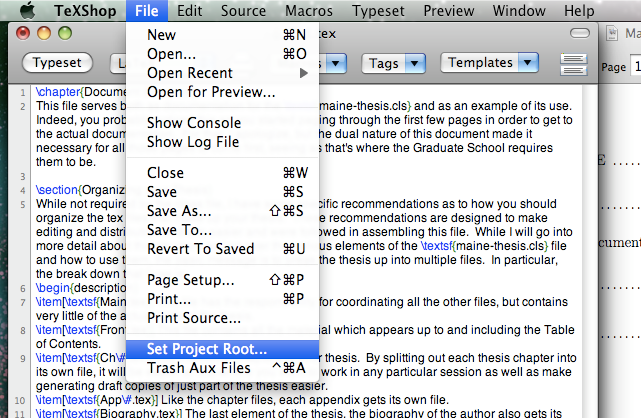
\includegraphics[height=2in]{Figures/ProjectRoot}
\caption[``Set Project Root...'' option in the File menu for TeXShop.]{``Set Project Root...'' option in the File menu for TeXShop.  This option is no longer a menu item in the most recent version of TeXShop but this figure is retained here as an example of figure usage.}
\label{rootmenu}
\end{figure}

\begin{figure}
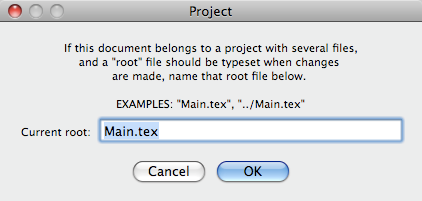
\includegraphics[height=2in]{Figures/Dialog}
\caption[``Set Project Root...'' dialog for TeXShop. ]{``Set Project Root...'' dialog for TeXShop.  This option is no longer a menu item in the most recent version of TeXShop but this figure is retained here as an example of figure usage.}
\label{rootdialog}
\end{figure}

If you're not using TeXShop or TeXWorks, then I suggest consulting the user manual or help files for your particular editor to figure out how to set the project root for a file.

\section{Organization of this document}
If you've read the Table of Contents, you've no doubt noticed that each of the chapters in this document deals with one of the files listed above.  In that chapter you'll find instructions for what has to be in that file.  For the most part these are requirements of either the Graduate School or the maine-thesis.cls itself.  Deviation from them may result in your document not typesetting correctly or in it not conforming to the Graduate School guidelines.  If you follow all these instructions perfectly and the Graduate School still rejects your thesis on the basis of some formatting error, please contact me (\email) with a full description of the problem that the Graduate School had with your thesis and I will make every effort to update the class file as quickly as possible.

\section{Reporting a Bug or Formatting Problem}
If you find a bug with this class file, please create a minimal working example which reproduces the bug and email it to \email\ along with a description of the bug and any possible fixes you have tried (and whether they worked or not).  For those not familiar with it, there are a couple of good descriptions on the web:
\begin{itemize}
\item{\url{http://www.tex.ac.uk/cgi-bin/texfaq2html?label=minxampl}}
\item{\url{http://www.minimalbeispiel.de/mini-en.html}}
\end{itemize}

If you find a formatting problem with this class file, please create a minimal working example which reproduces the problem and email it to \email\ along with a description of the formatting problem.  If the problem was pointed out to you by the Graduate School, please indicate who in the Graduate School pointed the problem so that I can consult with them directly if needed.  If available, a document which demonstrates what the desired formatting looks like should also be included.

I cannot guarantee any timeline on how quickly bugs or formatting problems will be dealt with, but I will make every effort to correct them as quickly as possible.

\endinput